\chapter{Results} 				
% File created 28-12-2016
\label{app:appendixG-Results}



\section{Order}
\label{sec:orderApp}


\begin{figure}
\centering
\subfloat[]{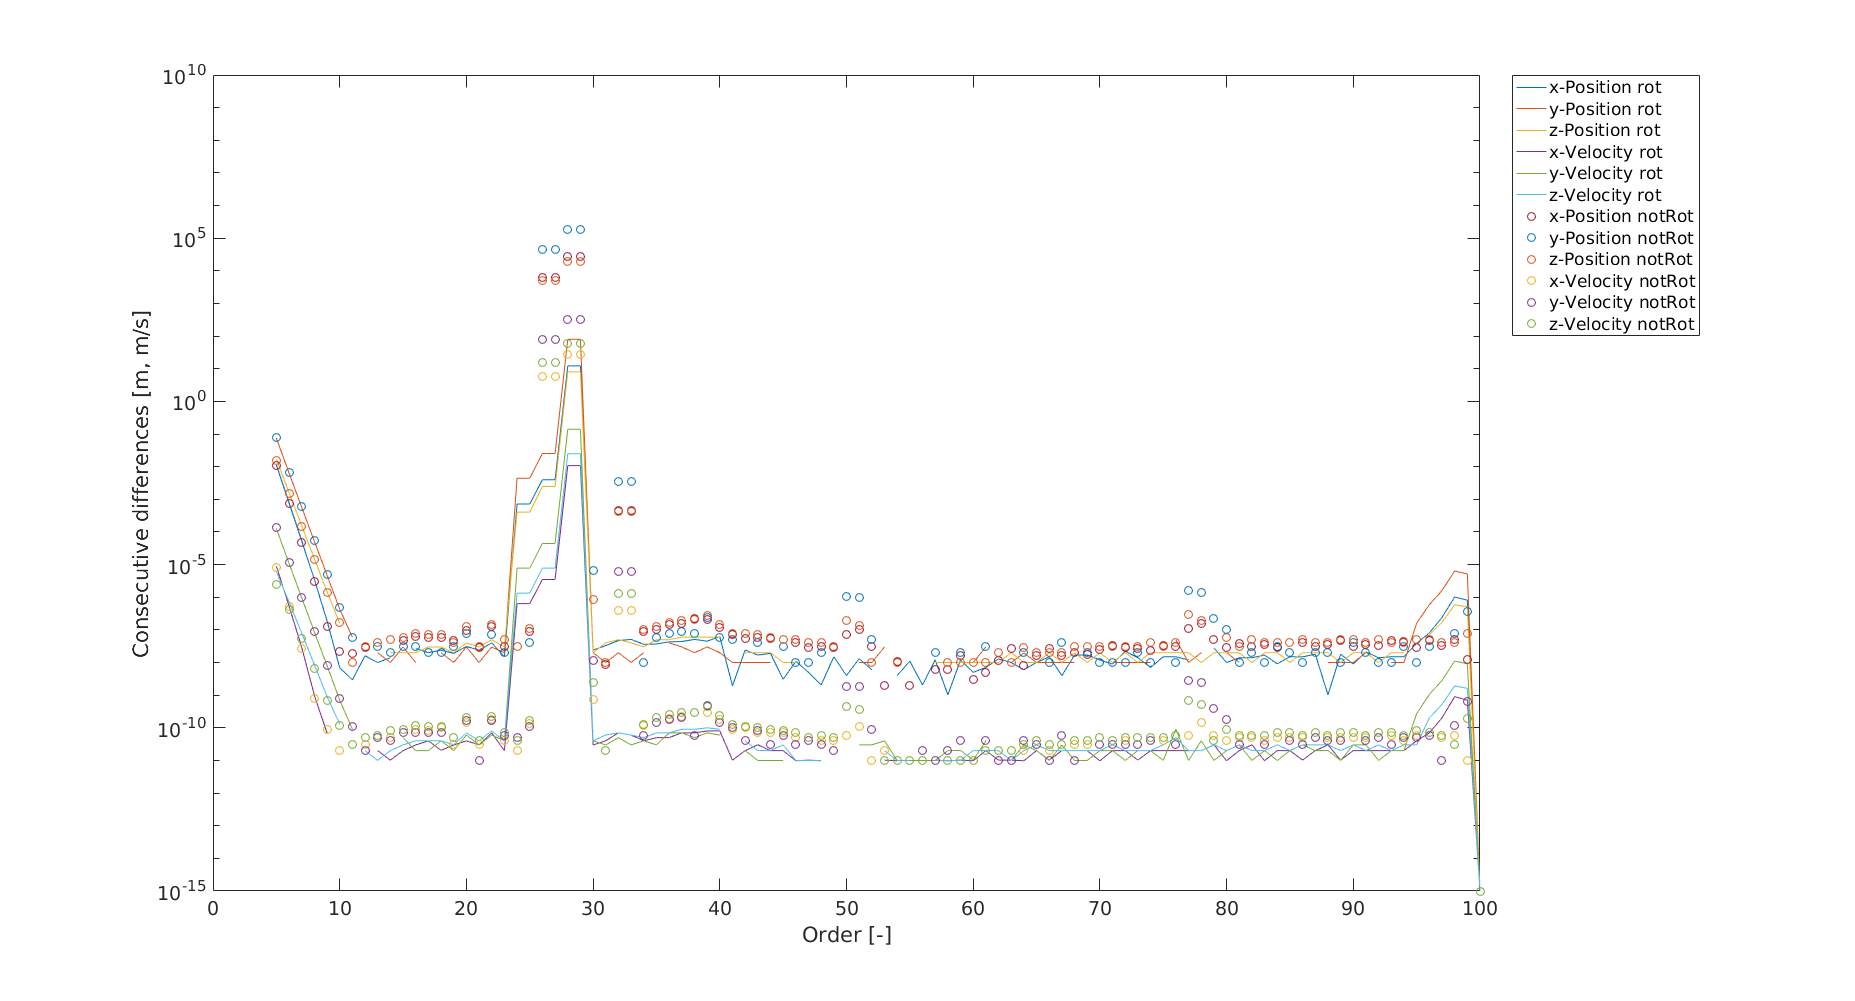
\includegraphics[width=1.1\textwidth]{figures/results/Order/orderVsConsecutiveDifferenceCase1combined.png}\label{subfig:orderVsConsecutiveDifferenceCase1combined}} \\

\subfloat[]{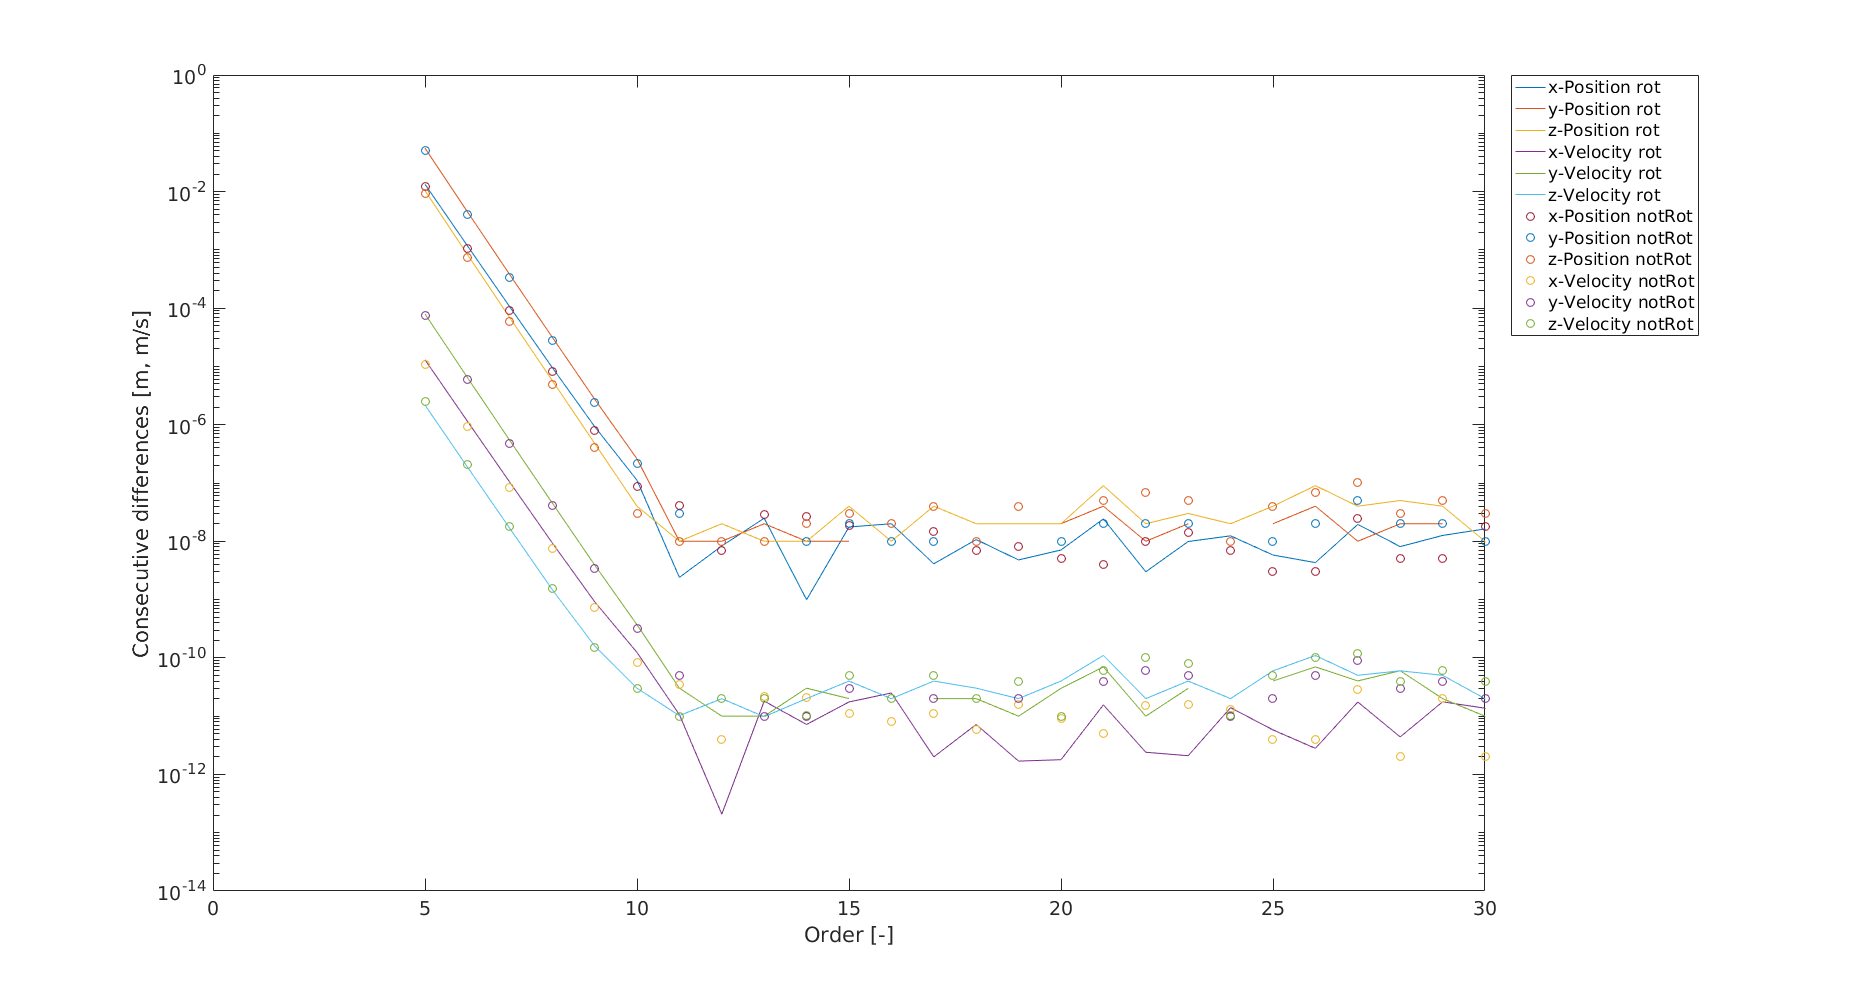
\includegraphics[width=1.1\textwidth]{figures/results/Order/orderVsConsecutiveDifferenceCase2combined.png}\label{subfig:orderVsConsecutiveDifferenceCase2combined}}
\caption{Consecutive difference for rotating and non-rotating Mars \protect\subref{subfig:orderVsConsecutiveDifferenceCase1combined} case 1, \protect\subref{subfig:orderVsConsecutiveDifferenceCase2combined} case 2 } 
\label{fig:orderVsConsecutiveDifferenceCase1combined} 
\end{figure} 

\begin{figure}
\centering
\subfloat[]{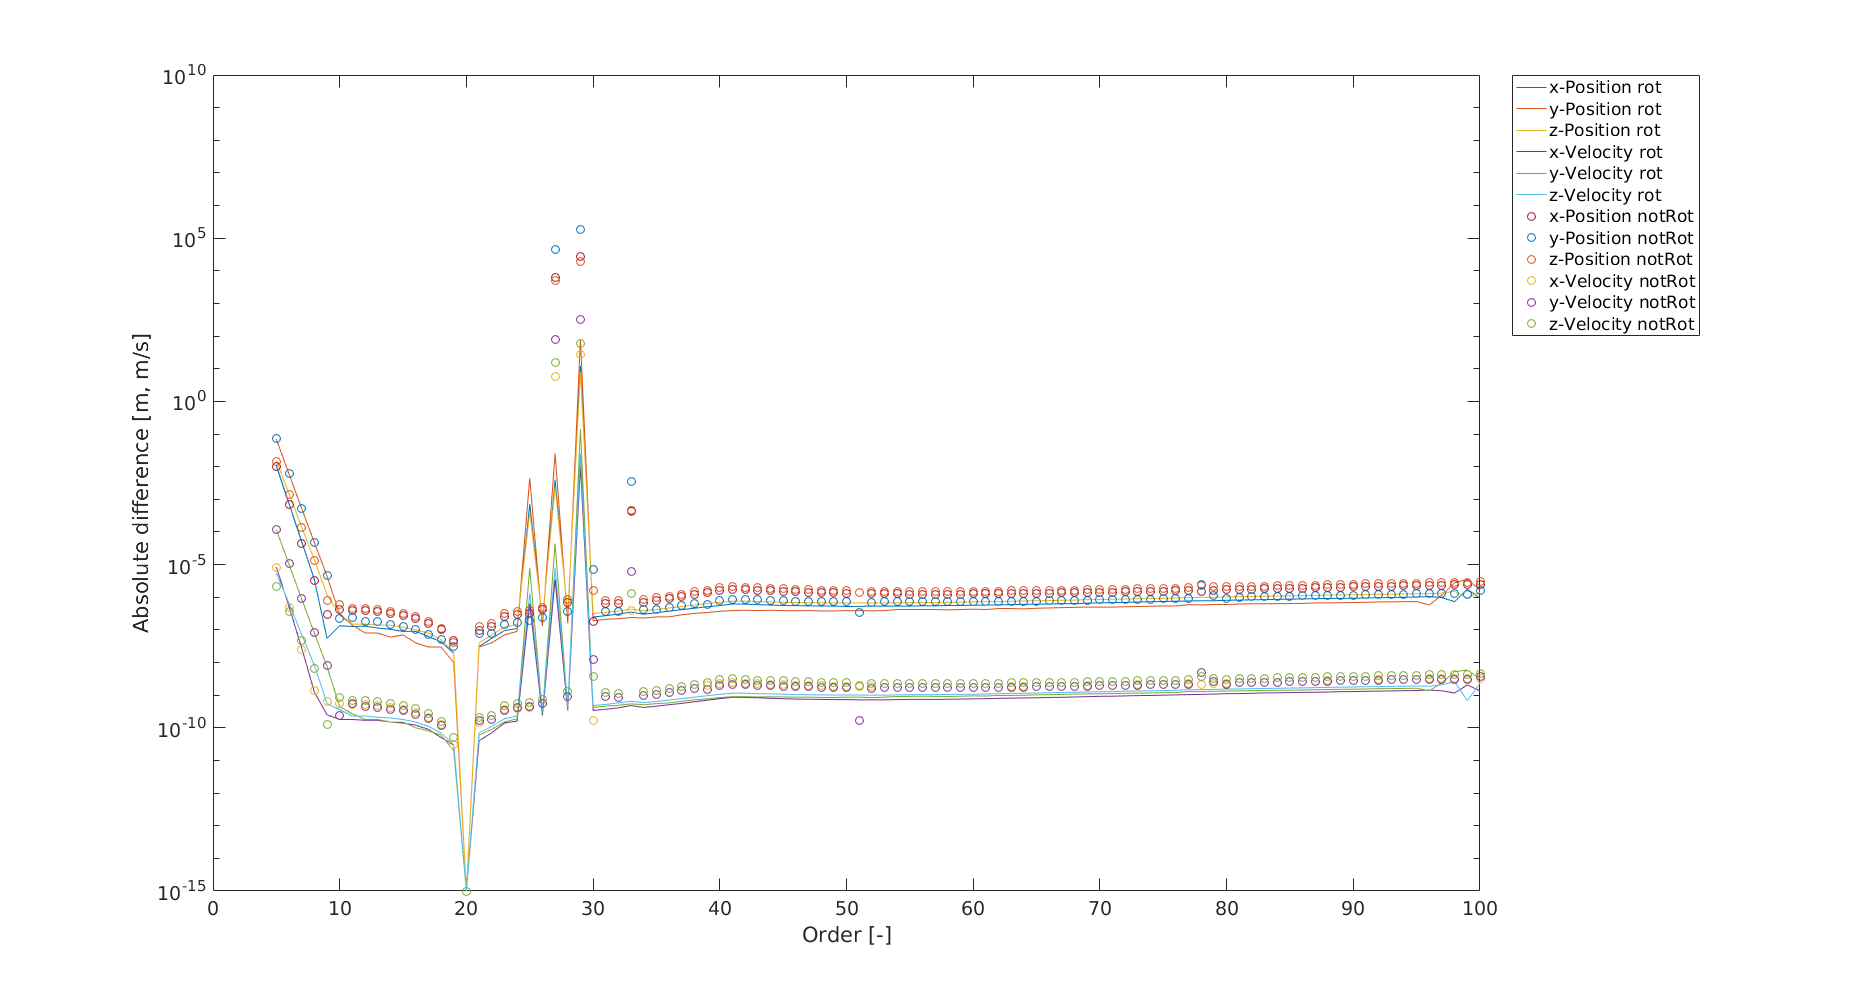
\includegraphics[width=1.2\textwidth]{figures/results/Order/orderVsNominalAbsoluteDifferenceCase1combined.png}\label{subfig:orderVsNominalAbsoluteDifferenceCase1combined}} \\

\subfloat[]{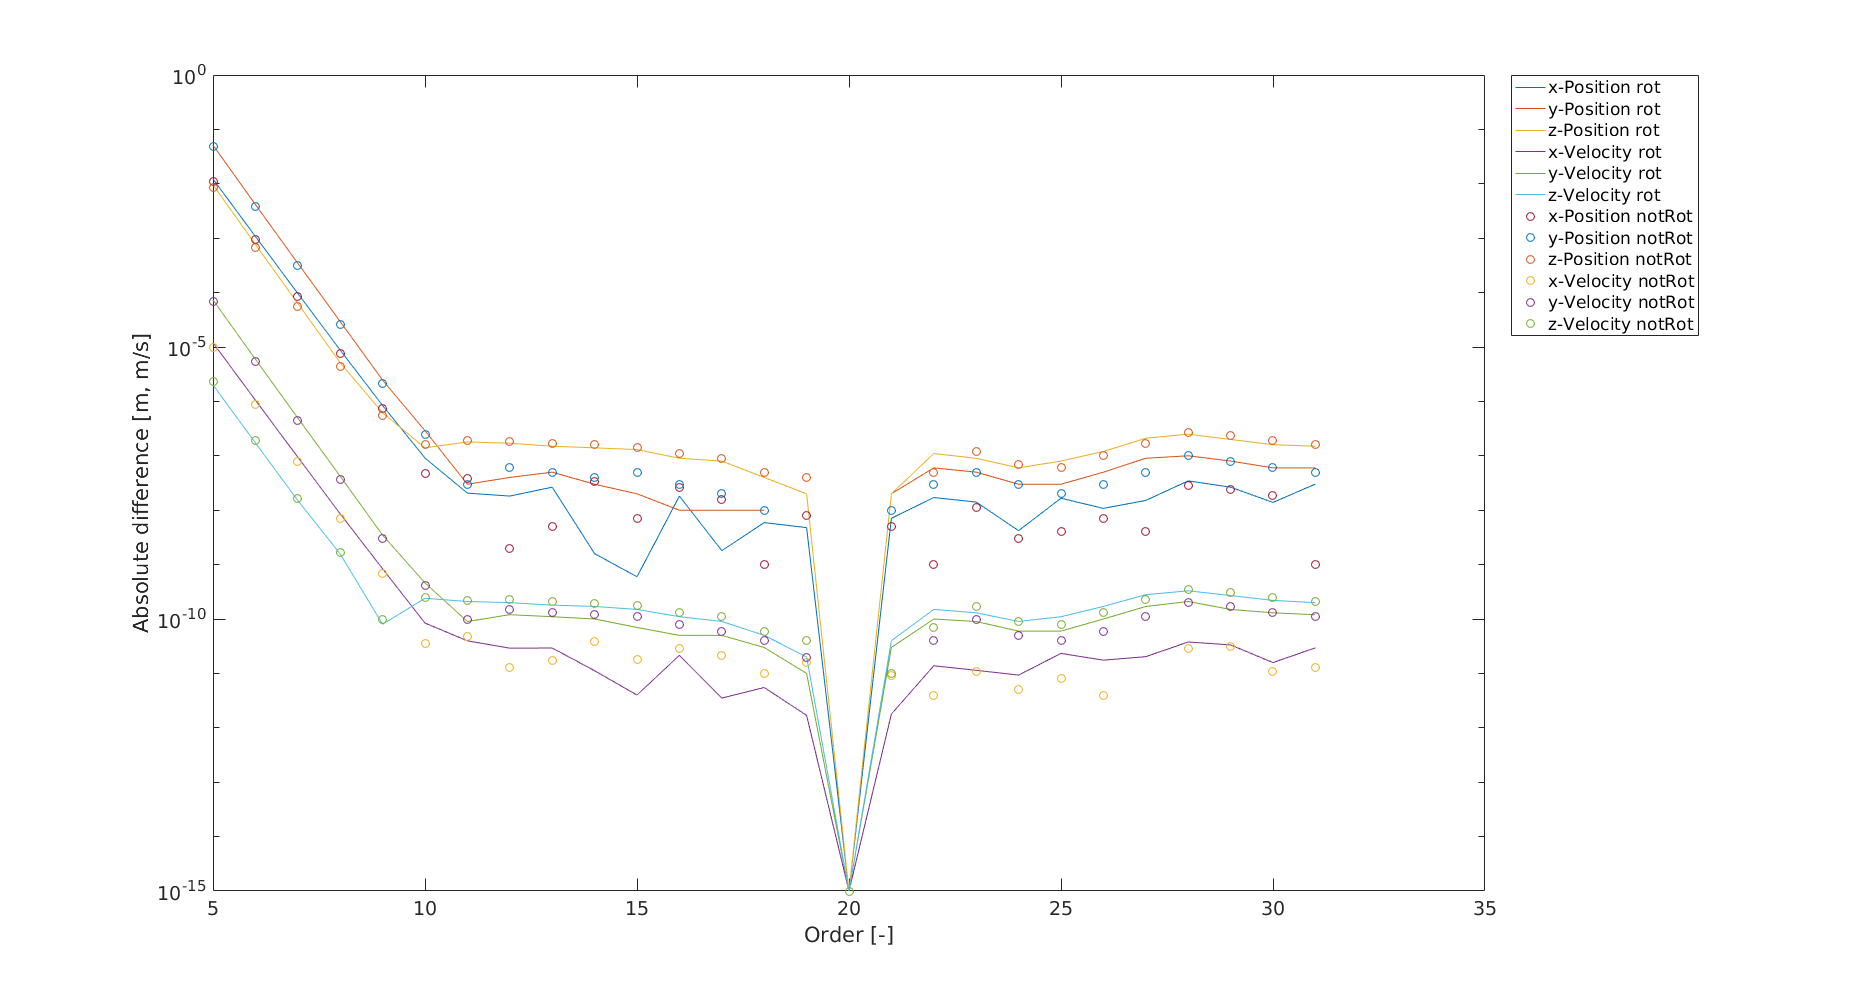
\includegraphics[width=1.2\textwidth]{figures/results/Order/orderVsNominalAbsoluteDifferenceCase2combined.png}\label{subfig:orderVsNominalAbsoluteDifferenceCase2combined}}
\caption{Difference with respect to the nominal case for rotating and non-rotating Mars \protect\subref{subfig:orderVsNominalAbsoluteDifferenceCase1combined} case 1, \protect\subref{subfig:orderVsNominalAbsoluteDifferenceCase2combined} case 2 } 
\label{fig:orderVsNominalAbsoluteDifferenceCase1combined} 
\end{figure}


\section{Error tolerance}
\label{sec:errorToleranceApp}


\section{Multiple runs}
\label{sec:multipleRunsApp}

\begin{figure}
\centering
\subfloat[]{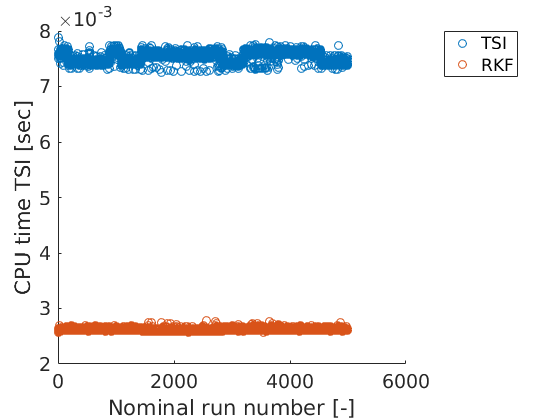
\includegraphics[width=3.1in]{figures/results/multiRun/multiRunVsCPUcase1RKFTSIsmall.png}\label{subfig:multiRunVsCPUcase1RKFTSI}} 
\subfloat[]{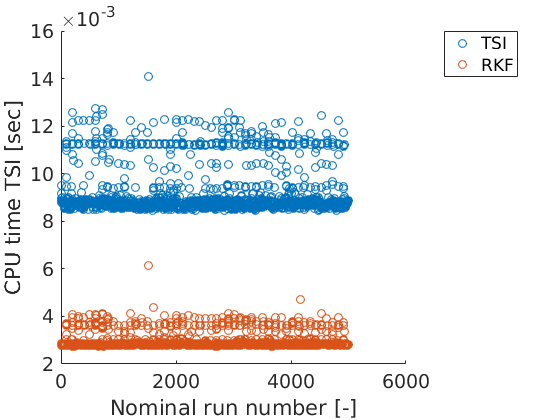
\includegraphics[width=3.1in]{figures/results/multiRun/multiRunVsCPUcase2RKFTSIsmall.png}\label{subfig:multiRunVsCPUcase2RKFTSI}}
\caption{Nominal runs versus CPU time comparison between \ac{RKF} and \ac{TSI} \protect\subref{subfig:multiRunVsCPUcase1RKFTSIsmall} case 1,  \protect\subref{subfig:multiRunVsCPUcase2RKFTSIsmall} case 2 } 
\label{fig:multiRunVsCPUcase1RKFTSI} 
\end{figure} 

\begin{figure}
\centering
\subfloat[]{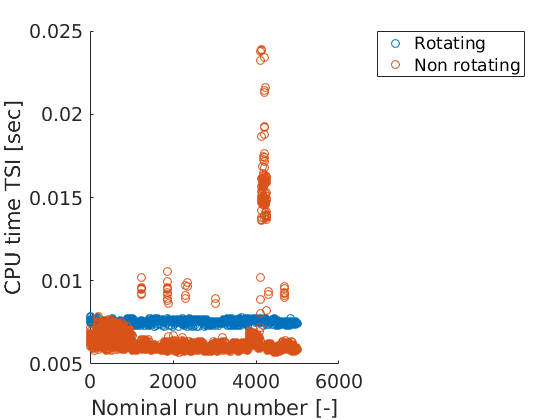
\includegraphics[width=3.1in]{figures/results/multiRun/multiRunVsCPUcase1combinedSmall.png}\label{subfig:multiRunVsCPUcase1combined}} 
\subfloat[]{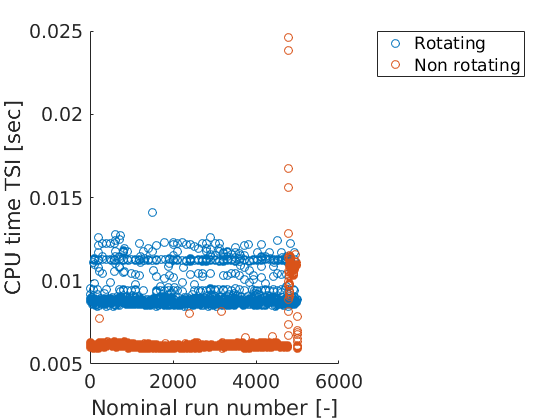
\includegraphics[width=3.1in]{figures/results/multiRun/multiRunVsCPUcase2combinedSmall.png}\label{subfig:multiRunVsCPUcase2combined}}
\caption{Nominal runs versus CPU time for rotating and non-rotating Mars \protect\subref{subfig:multiRunVsCPUcase1combinedSmall} case 1,  \protect\subref{subfig:multiRunVsCPUcase2combinedSmall} case 2 } 
\label{fig:multiRunVsCPUcase1combined} 
\end{figure} 


\section{Launch altitude}
\label{sec:launchAltitudeApp}

\section{Launch latitude}
\label{sec:launchLatitudeApp}

\section{Launch longitude}
\label{sec:launchLongitudeApp}

\section{Flight-path angle}
\label{sec:flightPathAngleApp}

\section{Heading angle}
\label{sec:headingAngleApp}